% ----------------------------------------------------
% Introduction
% ----------------------------------------------------
\documentclass[class=report,11pt,crop=false]{standalone}
% Page geometry
\usepackage[a4paper,margin=20mm,top=25mm,bottom=25mm]{geometry}

% Font choice
\usepackage{lmodern}

% Wrap text around image
\usepackage{wrapfig}

% Checkmarks
\usepackage{tikz}

% For algorithms
\usepackage[]{algorithm}
% Pseudocode packages
\usepackage{algpseudocode}

% Table color
% \usepackage{colortbl}

% Multiple rows
\usepackage{multirow}

% Lorem ipsum
\usepackage{lipsum}

% Use IEEE bibliography style
\bibliographystyle{IEEEtran}

% Line spacing
\usepackage{setspace}
\setstretch{1.20}

% Ensure UTF8 encoding
\usepackage[utf8]{inputenc}

% Language standard (not too important)
\usepackage[english]{babel}

% Skip a line in between paragraphs
\usepackage{parskip}

% For the creation of dummy text
\usepackage{blindtext}

% Math
\usepackage{amsmath}

% Lists
\usepackage{enumitem}

% Header & Footer stuff
\usepackage{fancyhdr}
\pagestyle{fancy}
\fancyhead{}
\fancyhead[R]{\nouppercase{\rightmark}}
\fancyfoot{}
\fancyfoot[C]{\thepage}
\renewcommand{\headrulewidth}{0.0pt}
\renewcommand{\footrulewidth}{0.0pt}
\setlength{\headheight}{13.6pt}

% Epigraphs
\usepackage{epigraph}
\setlength\epigraphrule{0pt}
\setlength{\epigraphwidth}{0.65\textwidth}

% Colour
\usepackage{color}
%\usepackage[usenames,dvipsnames]{xcolor}

% Hyperlinks & References
\usepackage{hyperref}
\definecolor{linkColour}{RGB}{77,71,179}
\hypersetup{
    colorlinks=true,
    linkcolor=linkColour,
    filecolor=linkColour,
    urlcolor=linkColour,
    citecolor=linkColour,
}
\urlstyle{same}

% Automatically correct front-side quotes
\usepackage[autostyle=false, style=ukenglish]{csquotes}
\MakeOuterQuote{"}

% Graphics
\usepackage{graphicx}
\graphicspath{{Images/}{../Images/}}
\usepackage{makecell}
\usepackage{transparent}

% SI units
\usepackage{siunitx}

% Microtype goodness
\usepackage{microtype}

% Listings
\usepackage[T1]{fontenc}
\usepackage{listings}
\usepackage[scaled=0.8]{DejaVuSansMono}

% Custom colours for listings
\definecolor{backgroundColour}{RGB}{250,250,250}
\definecolor{commentColour}{RGB}{73, 175, 102}
\definecolor{identifierColour}{RGB}{196, 19, 66}
\definecolor{stringColour}{RGB}{252, 156, 30}
\definecolor{keywordColour}{RGB}{50, 38, 224}
\definecolor{lineNumbersColour}{RGB}{127,127,127}
\lstset{
  language=Matlab,
  captionpos=b,
  aboveskip=15pt,belowskip=10pt,
  backgroundcolor=\color{backgroundColour},
  basicstyle=\ttfamily,%\footnotesize,        % the size of the fonts that are used for the code
  breakatwhitespace=false,         % sets if automatic breaks should only happen at whitespace
  breaklines=true,                 % sets automatic line breaking
  postbreak=\mbox{\textcolor{red}{$\hookrightarrow$}\space},
  commentstyle=\color{commentColour},    % comment style
  identifierstyle=\color{identifierColour},
  stringstyle=\color{stringColour},
   keywordstyle=\color{keywordColour},       % keyword style
  %escapeinside={\%*}{*)},          % if you want to add LaTeX within your code
  extendedchars=true,              % lets you use non-ASCII characters; for 8-bits encodings only, does not work with UTF-8
  frame=single,	                   % adds a frame around the code
  keepspaces=true,                 % keeps spaces in text, useful for keeping indentation of code (possibly needs columns=flexible)
  morekeywords={*,...},            % if you want to add more keywords to the set
  numbers=left,                    % where to put the line-numbers; possible values are (none, left, right)
  numbersep=5pt,                   % how far the line-numbers are from the code
  numberstyle=\tiny\color{lineNumbersColour}, % the style that is used for the line-numbers
  rulecolor=\color{black},         % if not set, the frame-color may be changed on line-breaks within not-black text (e.g. comments (green here))
  showspaces=false,                % show spaces everywhere adding particular underscores; it overrides 'showstringspaces'
  showstringspaces=false,          % underline spaces within strings only
  showtabs=false,                  % show tabs within strings adding particular underscores
  stepnumber=1,                    % the step between two line-numbers. If it's 1, each line will be numbered
  tabsize=2,	                   % sets default tabsize to 2 spaces
  %title=\lstname                   % show the filename of files included with \lstinputlisting; also try caption instead of title
}

% Caption stuff
\usepackage[hypcap=true, justification=centering]{caption}
\usepackage{subcaption}

% Glossary package
% \usepackage[acronym]{glossaries}
\usepackage{glossaries-extra}
\setabbreviationstyle[acronym]{long-short}

% For Proofs & Theorems
\usepackage{amsthm}

% Maths symbols
\usepackage{amssymb}
\usepackage{mathrsfs}
\usepackage{mathtools}

% For algorithms
%\usepackage[]{algorithm2e}

% Spacing stuff
\setlength{\abovecaptionskip}{5pt plus 3pt minus 2pt}
\setlength{\belowcaptionskip}{5pt plus 3pt minus 2pt}
\setlength{\textfloatsep}{10pt plus 3pt minus 2pt}
\setlength{\intextsep}{15pt plus 3pt minus 2pt}

% For aligning footnotes at bottom of page, instead of hugging text
\usepackage[bottom]{footmisc}

% Add LoF, Bib, etc. to ToC
\usepackage[nottoc]{tocbibind}

% SI
\usepackage{siunitx}

% For removing some whitespace in Chapter headings etc
\usepackage{etoolbox}
\makeatletter
\patchcmd{\@makechapterhead}{\vspace*{50\p@}}{\vspace*{-10pt}}{}{}%
\patchcmd{\@makeschapterhead}{\vspace*{50\p@}}{\vspace*{-10pt}}{}{}%
\makeatother
\makenoidxglossaries

\newacronym{radar}{RADAR}{Radio Detection and Ranging}
\begin{document}
	% ----------------------------------------------------
	\chapter{Methodology \label{ch:meth}}
	%\epigraph{Philosophers have hitherto only interpreted the world in various ways; the point is to change it.}%
	%    {\emph{---Karl Marx}}
	%\vspace{0.5cm}
	% ----------------------------------------------------
	
	%\lipsum[1]
	\section{Methodology Outline}
	
	This chapter details the design process and approach employed in achieving the aim of the project which is to  digitize and modernize the HP141T display by replacing the \acrshort{crt} monitor with a \acrshort{lcd} touchscreen display that offers different functions and modes of operation. Design decision are also documented here, showing the considerations that were made based on the operation and outputs of the HP141T spectrum analyzer and ensuring that the newly integrated display is compatible with the device's hardware. For example, the design required selection of the digital hardware for processing the analog voltage signals from the \acrshort{sa}. The selection of the digital processor made from single-board computers such as the Raspberry Pi 4 Model B, microcontrollers like the STM32F4 boards, \acrshort{fpga} such as the Artix-7 from Xilinix, or a heterogeneous digital processor which consists of a combination of these options. 
	
	Other considerations were made regarding the electronic circuits for converting the auxiliary output voltages from the HP141T to the appropriate voltage level for the operation of \acrshort{adc}. This chapter describes how together, the \acrshort{adc} and digital processor form a crucial part of the system. Additionally, the chapter details the software development kit (\acrshort{sdk}) and associated coding language that was used. The selection of the development framework depended on the choice of processor and digital processing algorithms that were required to fulfil the project requirements. For example, assuming that a \acrshort{fpga} is the chosen digital processor, the  \acrshort{sdk} would include tools such as the AMD Vivado and electronic design automation (\acrshort{eda}) software and the choice of coding language between Verilog, VHDL, and SystemVerilog would depend on how comfortable the developer is in representing digital processing algorithms, such the \acrshort{dft}, using the chosen language. 
	
	Overall, this chapter documents an overview of the design methodology and different phases in the design process. The design process followed a variation of V-Model in which a series of iterative phases was implemented with a process checking mechanism. The chapter begins by highlighting the design stages and modularization of the system. Thereafter, the chapter includes an assessment of the project requirements detailed in introductory section. Finally, the chapter describes the use of findings from the review of requirements in informing the design decisions and specifications.  
	
	\section{Phases in the Design Process}
	
	The design process was decomposed into four iterative stages as illustrated in Figure \ref{fig:design-stages-diagram} below. The first stage documented the digitization requirements and listed examples of modern \acrshort{sa}s in order to define the requirements for modernization. As shown in the methodology overview diagram, the first stage also included thorough investigation into methods that have been implemented in literature for upgrading the functions and performance of \acrshort{sa}s. A theoretical framework for relevant information about signal processing was also formulated based on the literature to ensure that the display modes and functions were consistent with the mathematically derived expected outputs in the system. 
	
	\begin{figure}[!ht]
		\centering
		\label{fig:design-stages-diagram}
		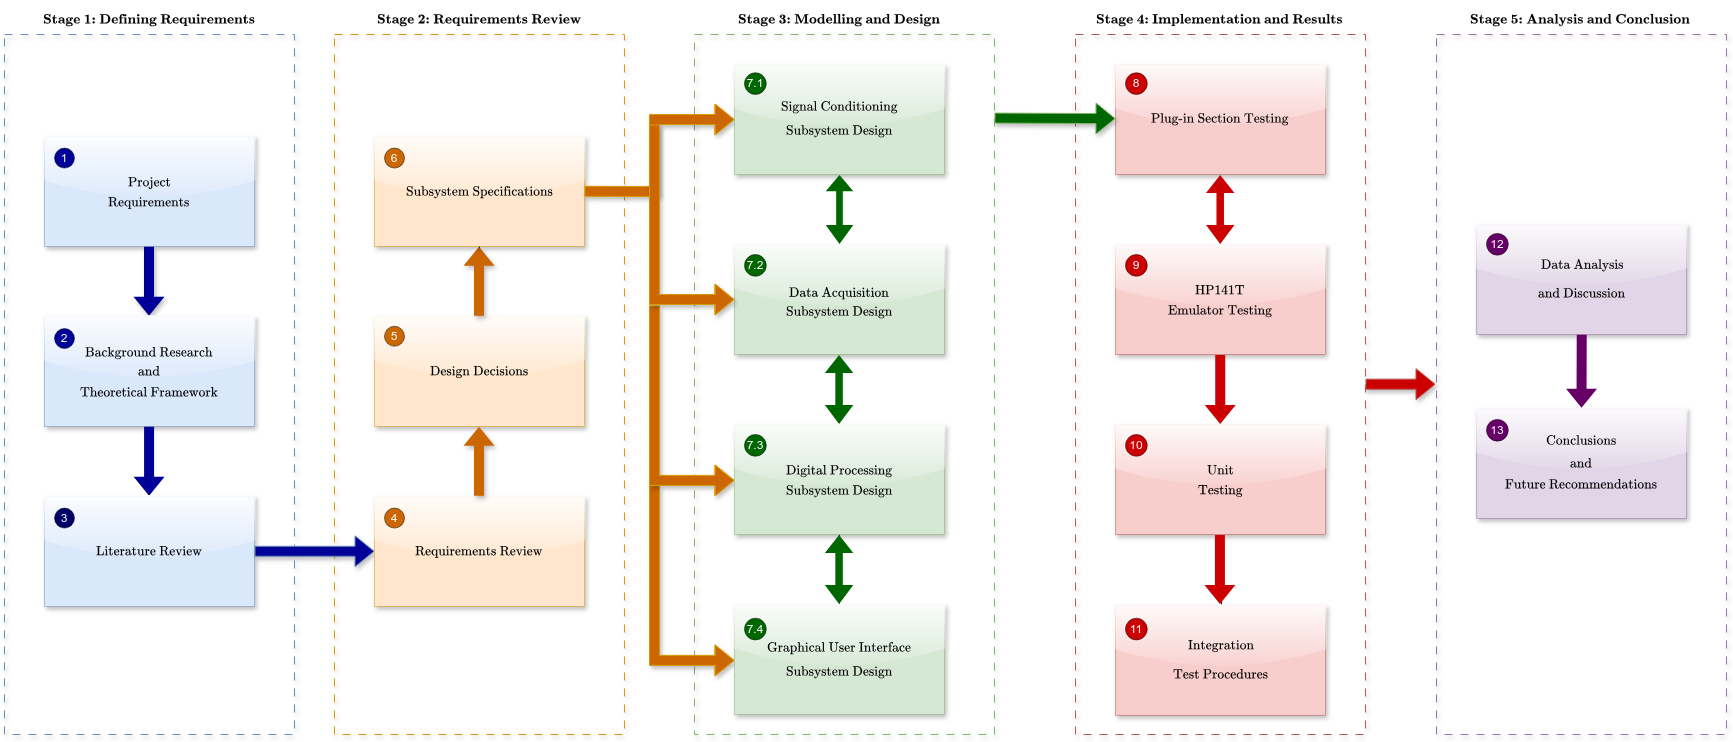
\includegraphics[width=1.0\linewidth]{Figures/Methodology/design-stages-diagram.png}
		\caption{Methodology overview showing different stages in the iterative design process that was applied as a variation of the V-Model.}
	\end{figure}
	
	The second stage in the design process involved a review of the user requirements specifications detailed in chapter \ref{ch:intro}. The aim of this step in the methodology was to clarify the desired functions of the upgraded spectrum analyzer and to inform the design decisions with respect to the digital hardware and software development for digital signal processing. Additionally, the requirements review was employed in modularizing the design into four subsystems including, the Analog-to-Digital Conversion, Digital Processing, Screen and User Interface subsystems. 
		
	Stage 3 of the design process dealt with the design specifications of each of these subsystems by further decomposing each module into smaller hardware and software components. Each function is tested against a requirement in Stage 4 where each design specification was verified and the operation of the integrated system was tested to ensure that the interfaces between the subsystems was configured correctly. 
	
	In general, implementation of the design process adhered to the following design steps detailed in the project brief and are associated with the user requirement specifications:
	
	\begin{enumerate}
		\item 
		Surveying the HP141T display and other outputs.
		\item 
		Surveying single-board computers and touchscreen options.
		\item 
		Phase One: establish a basic XYZ replica or HP141T emulator.
		\item 
		Phase Two: implement averaging and peak hold options.
		\item 
		Phase Three: annotate display axes.
		\item 
		Phase Four: determine the appropriate instrument settings. 
		\item 
		Phase Five: design new annotations for display taking instrument or operator manual inputs into account.
		\item 
		Phase Six: include more tutorial and operational instructions using.
	\end{enumerate}
	
	In finalizing the design process of the upgraded \acrshort{sa}, results from acceptance tests were assimilated and a conclusion was drawn. Then, based on the outcomes of the project, future recommendations were made for future iterations of the upgrade \acrshort{sa} system. Overall, the stages of the methodology included:
	
	\begin{itemize}
		\item 
		Stage 1: Defining Requirements
		\item 
		Stage 2: Requirements Review and System Overview
		\item 
		Stage 3: Modelling and Design
		\item 
		Stage 4: Implementation and Results
		\item 
		Stage 5: Analysis and Conclusion 
	\end{itemize}

	The first four stages of the design process were performed iteratively as a variation of the V-Model in which risk analysis was performed at each step, similar to the Spiral Model for design processes. Each iteration aimed at producing a new version of the upgraded HP141T display and a single conclusion was made when a satisfactory prototype was established.

	\section{Requirements Review}
	
	This section aims to clarify the scope and formalization of the user requirements specifications of the project. 
		
	\subsection{Comparing the HP141T System to Modern Spectrum Analyzer Displays}
	
	The first user requirement deals with the modernization of the HP141T system. The aim of this section is to review this requirement and to give clarification on the context of the use of "modernization" in this project. To achieve this objective, the section begins with a description of the HP141T system and the functions that differ from "modern" spectrum analyzers, such as the range of hand-held \acrshort{sa}s by FieldFox, and the N9000B CXA \acrshort{sa} manufactured by Keysight\textregistered. The section concludes with a summary table comparing the features of the HP141T system and modern spectrum analyzers. 
	
	The HP141T system is equipped with three plug-ins, namely the 8555A \acrshort{rf} section which operates in the microwave region of the electromagnetic spectrum, the 8552B \acrshort{if} section and the Model 141T display which includes the \acrshort{crt} monitor. The three plug-ins operate in unison to electronically scan signals in the time-domain and provide a visual representation of the input signal's amplitude in the frequency domain on the \acrshort{crt} monitor \cite{HP8555A}. Amplitude can be represented on a logarithmic ($\si{\decibel\meter}$) or linear scale ($\si{\milli\volt}$). 
	
	The 8555A and 8552B plug-ins apply principles of heterodyning spectroscopy, allows high frequency input signals with frequencies in the K-band of the microwave portion of the electromagnetic spectrum (i.e. $\SI{18}{\mega\hertz}$) \cite{harris2003}. Spectrum analyzers which rely on the \acrshort{fft} by sampling the continuous input signal and performing the Fourier transform on $N$ total samples typically deal with signals that have lower frequencies. This is because \acrshort{sa}s that employ the heterodyne principle like the HP141T determine the spectrum directly by analysis in the frequency domain and not from the time-dependent characteristics of the input signal. This is achieved by using a heterodyne receiver comprised of a mixer and tunable local oscillator (\acrshort{lo}) which convert the input signal to an intermediate frequency as illustrate in figure \ref{fig:heterodyne-rauscher} \cite{rauscher2007}. 
	
	\begin{figure}[!ht]
		\centering
		\label{fig:heterodyne-rauscher}
		
\includegraphics[width=0.3\linewidth]{Figures/Methodology/empty-image.png}
		\caption{Heterodyne Spectrum Analyzer Block Diagram.}
	\end{figure}
	
	In most cases, modern \acrshort{sa}s are real-time spectrum analyzers which are a special case of vector spectrum analyzers (\acrshort{vsa}) that use the heterodyne principle but digitize the input signal at the intermediate frequency, as shown in Figure \ref{fig:vector-analyzer-rover}, using a bandpass filter which can behave like a pre-select filter to limit distortions that arise from the mixer and shows the result in real-time. The advantage of digitizing the output of the \acrshort{if} section is that it enables large a input range of up to $\SI{50}{\mega\hertz}$ which can be analyzed in the time and frequency domain using digital signal processing techniques \cite{rovers2006}. Much like \acrshort{fft} analyzers, vector analyzers are limited by the minimum and maximum sampling rate at which the \acrshort{adc} can operate. Additionally, exceedingly high sampling rates can lead to aliasing which causes frequencies outside of the bandwidth to fold into the frequency band \cite{rovers2006}. 	

	\begin{figure}[!ht]
		\centering
		\label{fig:vector-analyzer-rover}
		
\includegraphics[width=0.3\linewidth]{Figures/Methodology/empty-image.png}
		\caption{Vector analyzer block diagram showing digitization of the \acrshort{if} frequency.}
	\end{figure}

	Examples of modern real-time analyzers include:
	
	\begin{itemize}
		\item 
		Tektronix RSA2208A which can scan input signals with frequencies of up to $\SI{8}{\giga\hertz}$.
		\item 
		Rohde \& Schwarz FSP13 which operates within a $\SI{9}{\giga\hertz}$ to $\SI{30}{\giga\hertz}$ \acrshort{rbw}.
		\item
		Agilent E4445A which offer frequency analysis up to $\SI{13.2}{\giga\hertz}$.
		\item 
		FieldFox RTSA which covers $\SI{5}{\kilo\hertz}$ up to $\SI{50}{\giga\hertz}$.
	\end{itemize}

	
	\subsection{Representation of Signals in Frequency Domain}
	
	\subsection{Spectrum Analyzer Modes of Operation}
	
	\subsection{Display Resolution in the Logarithmic Scale}
	
	\subsection{Components of the Software Development Kit}
	
	\subsection{Display Power Source}
	
	\subsection{Equipment for Debugging and Testing}
		
	\section{System Design}
	
	\subsection{System Modularization}
	
	\subsection{System Block Diagrams}
	% ----------------------------------------------------
	\ifstandalone
	\bibliography{../Bibliography/References.bib}
	\printnoidxglossary[type=\acronymtype,nonumberlist]
	\fi
\end{document}
% ----------------------------------------------------